\subsection{List of enrolled students Page}
The Insert Rides Page contains the form necessary to insert a new ride.\\

There is a static and a dynamic part of the page. In the static part, it is possible to insert the description of the ride, the park it is going to be deployed in and its model. Both the park input and the model input are going to be filled automatically, based on the data available in the database.\\

Dynamic aspects of the page regard the possibility of adding (and removing) on the fly additional devices that are mounted on the ride. By clicking on a “+” button, a new device form will be inserted in the device form area. There is also a “-” button, which will allow the user to remove devices. Note that, each device form will have its own “-” button. This way, the user can remove specific devices, without the need for additional effort that might stem from the removal of the last inserted device.\\

Upon completion, if the insertion ended correctly, the user is redirected to the homepage.

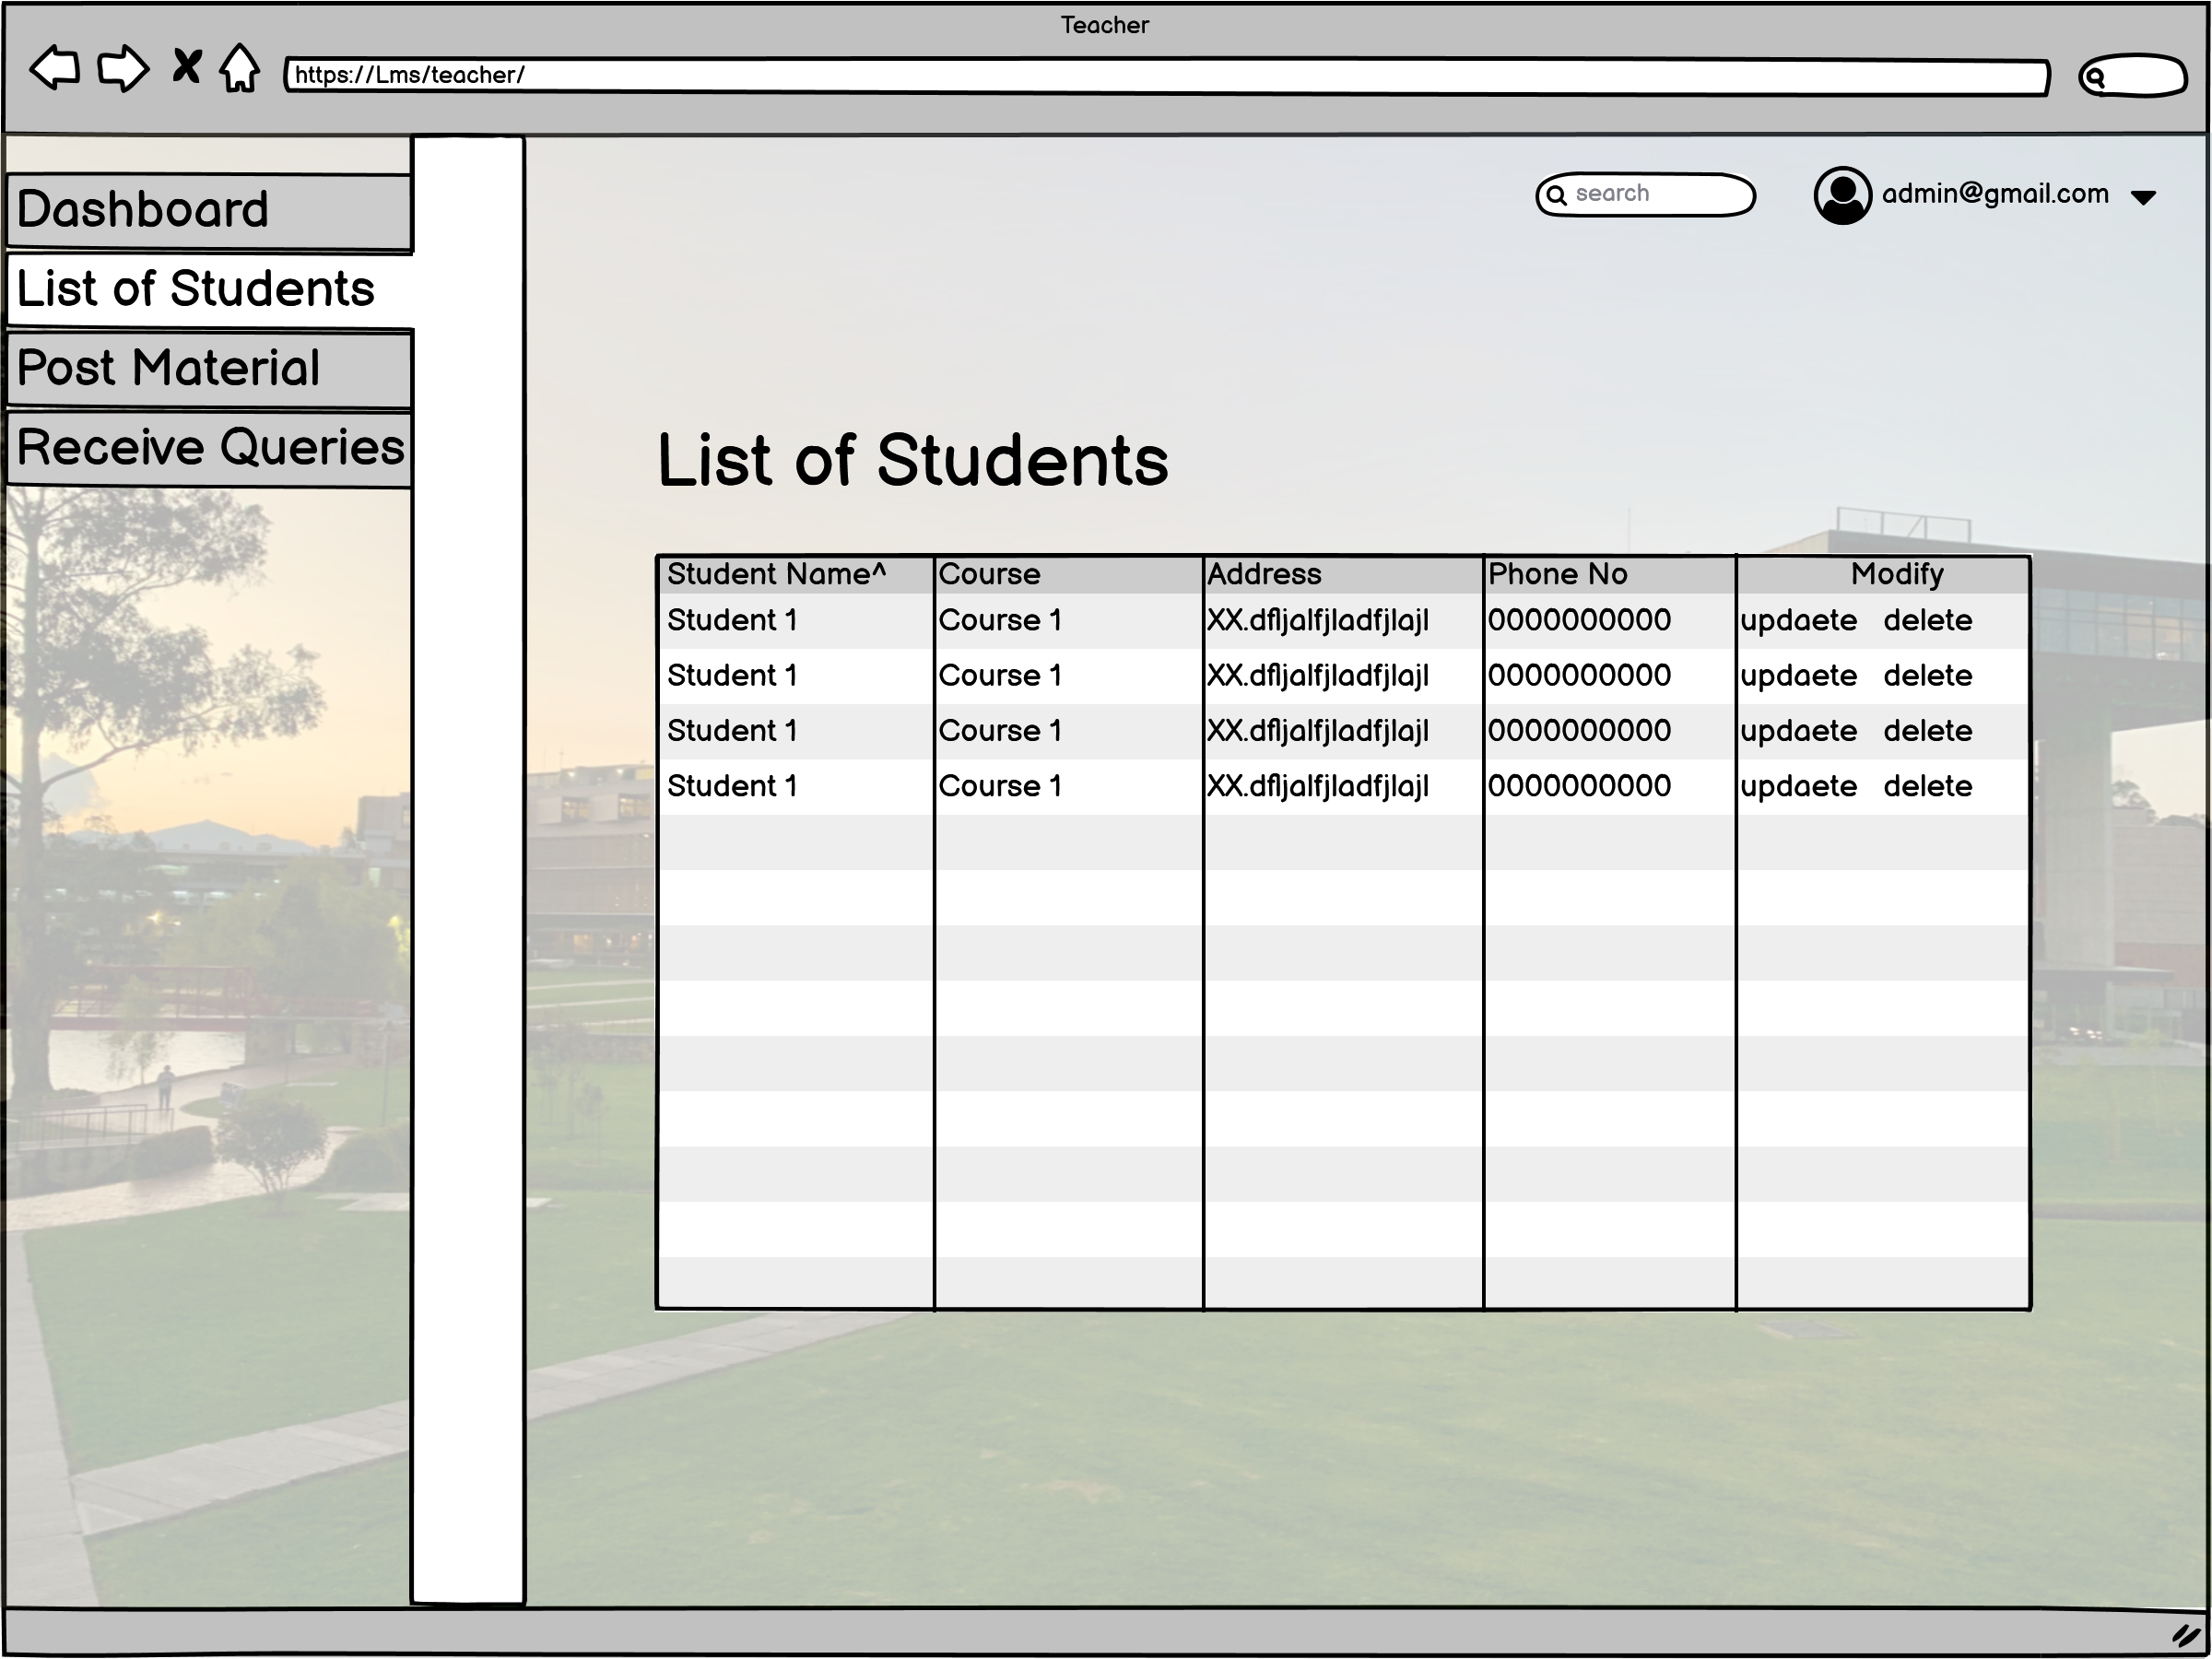
\includegraphics[width=\columnwidth]{images/List of Students teacher.png}